\documentclass[a4paper,openright,12pt]{report}
\usepackage[spanish]{babel} % espanol
\usepackage[latin1]{inputenc} % acentos sin codigo
\usepackage{graphicx} % graficos
\usepackage{hyperref}
\usepackage[utf8]{inputenc}

\begin{document}
\begin{titlepage}
%CARATULA
\begin{center}
\vspace*{-1in}
\begin{figure}[htb]
\begin{center}

\includegraphics[width=4cm]{./images/upt}
\end{center}
\end{figure}

UNIVERSIDAD PRIVADA DE TACNA\\
\vspace*{0.15in}
FACULTAD DE INGENIERIA\\
Escuela Profesional de Ingeniería de Sistemas\\
\vspace*{0.6in}
\begin{large}
TEMA : \\
\end{large}
\vspace*{0.2in}
\begin{Large}
\textbf{ALBERT EINSTEIN} \\
\end{Large}
\vspace*{0.3in}
\begin{large}
DOCENTE: PATRICK CUADROS QUIROGA\\
\end{large}
\vspace*{0.3in}
\rule{80mm}{0.1mm}\\
\vspace*{0.1in}
\begin{large}
PRESENTADO POR: \\
Jose Luis Condori Choquecota \\
\end{large}
\vspace*{2in}
\begin{large}
2017\\
\end{large}
\end{center}
%CARATULA
%INDICE




\tableofcontents
\begin{large}
\chapter{Biografia}
\begin{flushleft}
Albert Einstein, nacido en Ulm, Alemania, el 14 de marzo de 1879 fue un físico nacionalizado posteriormente estadounidense. Está considerado como el científico más importante del siglo XX, además de ser el más conocido.\\

Hombre tremendamente despistado, inconformista, muy consciente de sus dotes excepcionales, ambicioso y enamorado de la belleza matemática. Cambió nuestra concepción del Universo, del espacio y del tiempo.\\
\end{flushleft}


\chapter{La Relatividad}\label{cap.nudo}
\begin{flushleft}
En el siglo XVII, la sencillez y elegancia con que Isaac Newton había logrado explicar las leyes que rigen el movimiento de los cuerpos y el de los astros, unificando la física terrestre y la celeste, deslumbró hasta tal punto a sus contemporáneos que llegó a considerarse completada la mecánica. A finales del siglo XIX, sin embargo, era ya insoslayable la relevancia de algunos fenómenos que la física clásica no podía explicar. Correspondió a Albert Einstein superar tales carencias con la creación de un nuevo paradigma: la teoría de la relatividad, punto de partida de la física moderna.\\
En tanto que modelo explicativo completamente alejado del sentido común, la relatividad se cuenta entre aquellos avances que, en los albores del siglo XX, conducirían al divorcio entre la gente corriente y una ciencia cada vez más especializada e ininteligible. No obstante, ya en vida del físico o póstumamente, incluso los más sorprendentes e incomprensibles aspectos de la relatividad acabarían siendo confirmados. No debe extrañar, pues, que Albert Einstein sea uno de los personajes más célebres y admirados de la historia de la ciencia: saber que son ciertas tantas ideas apenas concebibles (por ejemplo, que la masa de un cuerpo aumenta con la velocidad) no deja más opción que rendirse a su genialidad.\\

\vspace*{0.6in}

\begin{center}
{\Large E=MC^2}
\end{center}
\end{flushleft}

\chapter{Fotos}\label{cap.desenlace}
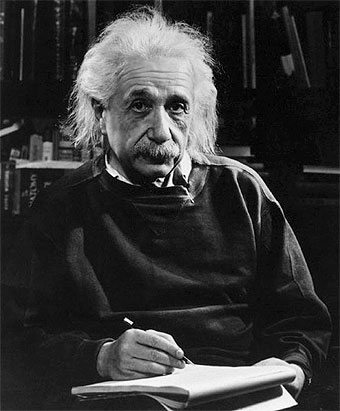
\includegraphics[width=4cm]{./images/1}
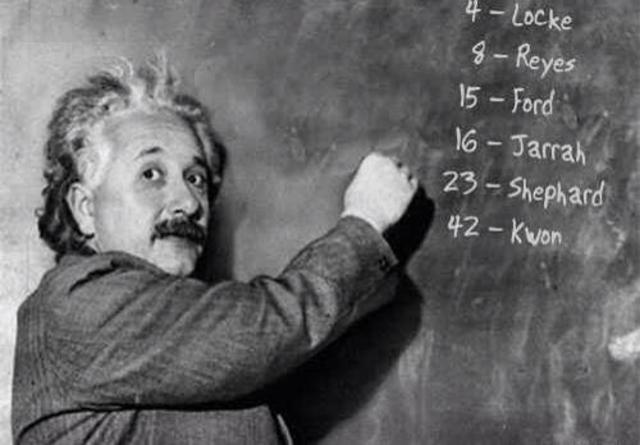
\includegraphics[width=7cm]{./images/2}
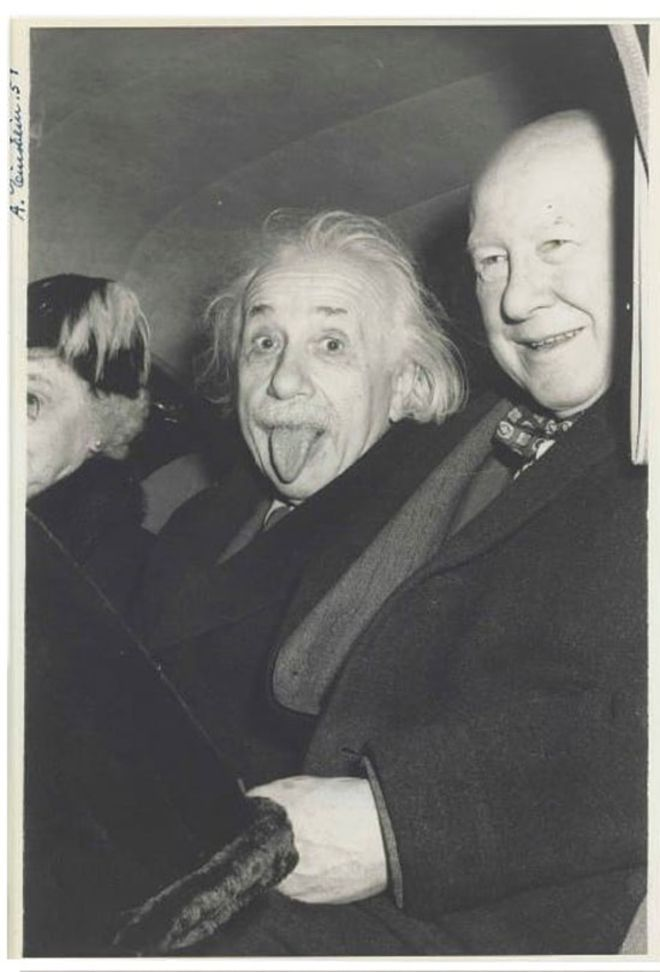
\includegraphics[width=3.5cm]{./images/3}



\end{large}
%FIN INDICE
%bibliografia
\begin{thebibliography}{X}
\bibitem{Baz} \textsc{Bazaraa, M.S., J.J. Jarvis} y \textsc{H.D. Sherali},
\textit{Programaci\’on lineal y flujo en redes}, segunda edici\’on,
Limusa, M\’exico, DF, 2004.

\end{thebibliography}
%fin bibliografia

\end{titlepage}

\end{document}
